\documentclass[t]{beamer}

%%%%%%%%%%%%%%%%%%%%%%%%%%%%%%
% Packages
%%%%%%%%%%%%%%%%%%%%%%%%%%%%%%

\usepackage{geometry}              		 % 
\usepackage[dutch]{babel}                % Voor nederlandstalige hyphenatie (woordsplitsing)
\uselanguage{dutch}
\languagepath{dutch}
\usepackage{amsmath,amsthm}              % Uitgebreide wiskundige mogelijkheden
\usepackage{url}                         % Om url's te verwerken
\usepackage{graphicx,subfigure}          % Om figuren te kunnen verwerken
\usepackage{color}						 % Om kleuren in Inkscape figuren te kunnen weergeven
\usepackage[utf8]{inputenc}              % Om niet ascii karakters rechtstreeks te kunnen typen
\usepackage{float}                       % Om nieuwe float environments aan te maken. Ook optie H!
\usepackage[section]{placeins}			 % Om ervoor te zorgen dat floats binnen dezelfde section blijven
\usepackage{eurosym}                     % om het euro symbool te krijgen
\usepackage{textcomp}                    % Voor onder andere graden celsius
%\usepackage{fancyhdr}                    % Voor fancy headers en footers
\usepackage{parskip}                     % Om paragrafen met een verticale spatie ipv horizontaal te laten beginnen
\usepackage{multicol}
%\usepackage[plainpages=false]{hyperref}  % Om hyperlinks te hebben in het pdfdocument
\usepackage[absolute,overlay]{textpos}

%%%%%%%%%%%%%%%%%%%%%%%%%%%%%%
% Layout
%%%%%%%%%%%%%%%%%%%%%%%%%%%%%%
\usetheme{Frankfurt}
\AtBeginSection[]
{
  \begin{frame}
    \frametitle{Inhoud}
    \tableofcontents[currentsection]
  \end{frame}
}

%%%%%%%%%%%%%%%%%%%%%%%%%%%%%%
% Omgevingen
%%%%%%%%%%%%%%%%%%%%%%%%%%%%%%


%%%%%%%%%%%%%%%%%%%%%%%%%%%%%%
% Nieuwe commandos
%%%%%%%%%%%%%%%%%%%%%%%%%%%%%%

% De differentiaal operator
\newcommand{\diff}{\ensuremath{\mathrm{d}}}
\newcommand{\subsdiff}{\ensuremath{\mathrm{D}}}
\newcommand{\vardiff}{\ensuremath{\mathrm{\delta}}}

% Super en subscript
\newcommand{\supsc}[1]{\ensuremath{^{\text{#1}}}}   % Superscript in tekst
\newcommand{\subsc}[1]{\ensuremath{_{\text{#1}}}}   % Subscript in tekst

% Vectoren en matrices
\newcommand{\vt}[1]{\ensuremath{\boldsymbol{#1}}} % vector in juiste lettertype
\newcommand{\mx}[1]{\ensuremath{\mathsf{#1}}}	  % matrix in juiste lettertype

% Nieuw commando om iets te benadrukken en tegelijkertijd in de index te steken.
\newcommand{\begrip}[1]{\index{#1}\textbf{#1}\xspace}

% Graden celcius
\newcommand{\degC}{\ensuremath{^\circ \mathrm{C}}}


% nieuw commando om svg files dynamisch te updaten
\newcommand{\executeiffilenewer}[3]{%
\ifnum\pdfstrcmp{\pdffilemoddate{#1}}%
{\pdffilemoddate{#2}}>0%
{\immediate\write18{#3}}\fi%
}
% nieuw commando om. svg figuren in te voegen
% Gebruik: \includesvg{path/filename.svg}
\newcommand{\includesvg}[2][0]{%
\executeiffilenewer{#2.svg}{#2.pdf}%
{inkscape -z -C --file=#2.svg %
--export-pdf=#2.pdf --export-latex}%
\ifx#10
	\let\svgwidth\undefined
\else
	\def\svgwidth{#1}
\fi%
\input{#2.pdf_tex}%
\ifx \svgwidth\undefined
\else
	\let\svgwidth\undefined
\fi%
}

% nieuw commando om .fig figuren in te voegen
\newcommand{\includefig}[2][0]{%
\ifx#10
	\let\figwidth\undefined
\else
	\def\figwidth{#1}
\fi%
\input{#2.pdf_tex}%
\ifx \figwidth\undefined
\else
	\let\figwidth\undefined
\fi%
}

\usepackage{amsmath,amsthm}             % Uitgebreide wiskundige mogelijkheden

%%%%%%%%%%%%%%%%%%%%%%%%%%%%%%
% Nieuwe commandos
%%%%%%%%%%%%%%%%%%%%%%%%%%%%%%

% De differentiaal operator
\newcommand{\diff}{\ensuremath{\mathrm{d}}}
\newcommand{\subsdiff}{\ensuremath{\mathrm{D}}}
\newcommand{\vardiff}{\ensuremath{\mathrm{\delta}}}

% Super en subscript
\newcommand{\supsc}[1]{\ensuremath{^{\text{#1}}}}   % Superscript in tekst
\newcommand{\subsc}[1]{\ensuremath{_{\text{#1}}}}   % Subscript in tekst

% Vectoren en matrices
\newcommand{\vt}[1]{\ensuremath{\boldsymbol{#1}}} % vector in juiste lettertype
\newcommand{\mx}[1]{\ensuremath{\mathsf{#1}}}	  % matrix in juiste lettertype

% Nieuw commando om iets te benadrukken en tegelijkertijd in de index te steken.
\newcommand{\begrip}[1]{\index{#1}\textbf{#1}\xspace}

% Graden celcius
\newcommand{\degC}{\ensuremath{^\circ \mathrm{C}}}
% graden
\renewcommand{\deg}{\ensuremath{^\circ}}

% unit
\newcommand{\unit}[1]{\ensuremath{\mathrm {#1}}}

\subtitle{Behoudsvergelijkingen langs stroomlijnen}

\begin{document}

	\frame{\titlepage}
	\section{Inleiding}
	\begin{frame}
		\frametitle{Voorbeeld}
		\center
    	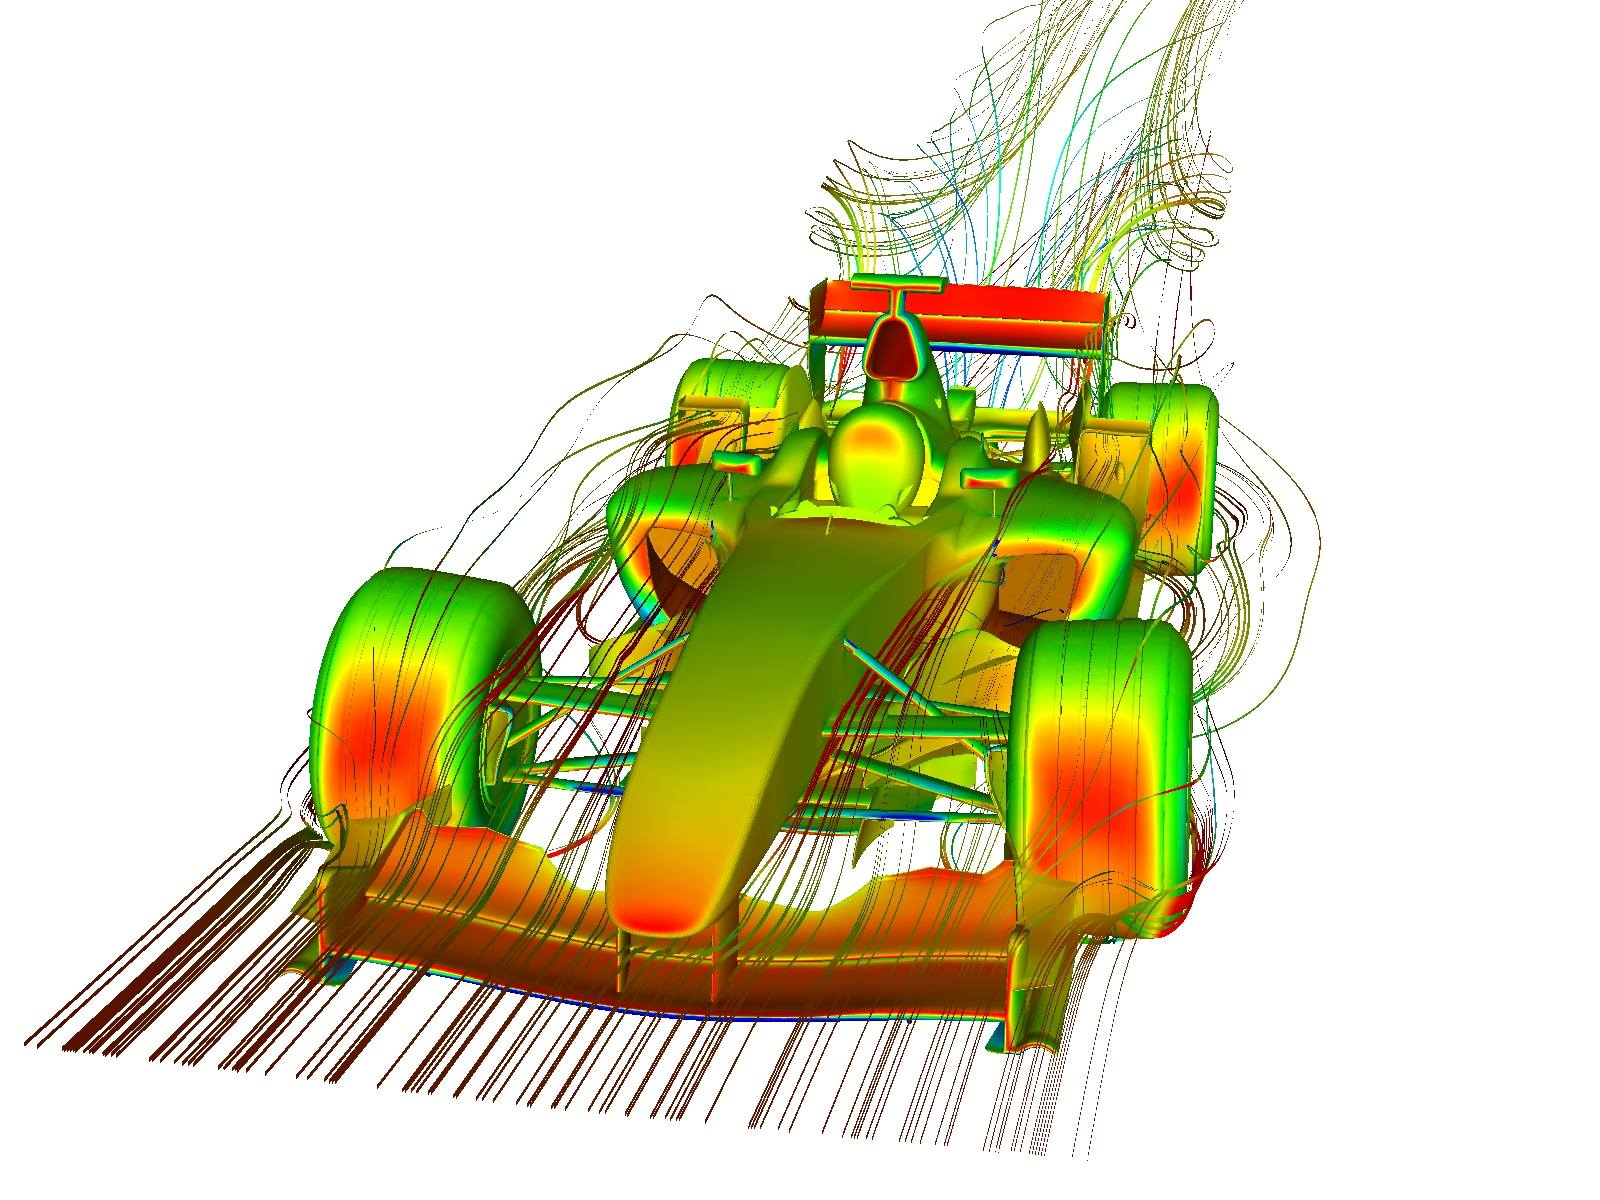
\includegraphics[height=0.8\textheight]{../fig/deeltjesvergelijkingen/Dalco_Supercomputer_CFD_BMW_F1_PressurePath.jpg}\\
		\footnotesize{Bron: http://www.dalco.ch/}
  	\end{frame}
%%%%%%%%%%%%%%%%%%%%%%%%%%%%%%%%%%%%%%%%%%%%%%%%%%%%%%%%%%%%%%%%%%%%%%%%%%%
  	\section{Bewegingsvergelijking}	
  	\begin{frame}
		\frametitle{Stroomlijncoordinaten}
		\vspace{0.5cm}
		\centering
		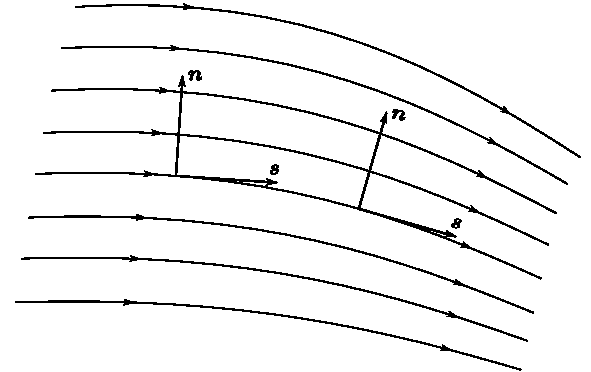
\includegraphics{../fig/deeltjesvergelijkingen/Stoomlijncoordinaten}
  	\end{frame}
 %%%%%%%%%%%%%%%%%%%%%%%%%%%%%%%%%%%%%%%%%%%%%%%%%%%%%%%%%%%%%%%%%%%%%%%%%%%
  	\begin{frame}
		\frametitle{Bewegingsvergelijking}
		\vspace{0.5cm}
		\centering
		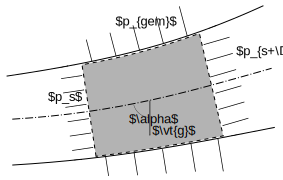
\includegraphics{../fig/deeltjesvergelijkingen/Controlevolume_tussen_stroomlijnen}
  	\end{frame}
%%%%%%%%%%%%%%%%%%%%%%%%%%%%%%%%%%%%%%%%%%%%%%%%%%%%%%%%%%%%%%%%%%%%%%%%%%%
  	\begin{frame}
		\frametitle{Bewegingsvergelijking}
		\begin{textblock}{5}(0,3)
            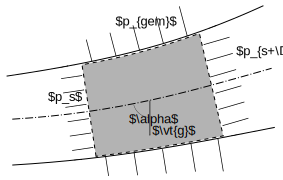
\includegraphics[width=5cm]{../fig/deeltjesvergelijkingen/Controlevolume_tussen_stroomlijnen}
        \end{textblock}
        \only<1-3>{
        	\vspace{2.5cm}
        	\begin{equation*}
				\frac{\diff \vt{P}_{CV}}{\diff t} + \dot{\vt{P}}_{\partial CV} =  \vt{F}
        	\end{equation*}
        }
        \only<2-3>{
        	\begin{align*}
				\left. \rho v v_{\perp} A \right|_{s+\Delta s} - \left. \rho v v_{\perp} A \right|_{s} &= \left. p A \right|_{s} - \left. p A \right|_{s+\Delta s} \\
				&+ p_{gem} (\left. A \right|_{s+\Delta s}-\left. A \right|_{s}) -\rho g A_{gem} \Delta s \cos \alpha
        	\end{align*}
        }
        \only<3-3>{
        	\begin{align*}
				\frac{\left. \rho v v A \right|_{s+\Delta s} - \left. \rho v v A \right|_{s}}{\Delta s} &= -\frac{\left. p A \right|_{s+\Delta s} - \left. p A \right|_{s}}{\Delta s} \\
				& + p_{gem} \frac{\left. A \right|_{s+\Delta s}-\left. A \right|_{s}}{\Delta s} -\rho g A_{gem} \frac{\left. z\right|_{s+\Delta s} - \left. z\right|_{s}}{\Delta s}
			\end{align*}
		}
		\only<4-6>{
			\vspace{3.5cm}
			\begin{equation*}
				\frac{\diff \rho v v A}{\diff s} = -\frac{\diff p A}{\diff s} + p \frac{\diff A}{\diff s} -\rho g A \frac{\diff z}{\diff s}
			\end{equation*}
		}
		\only<5-6>{
			\begin{equation*}
				\rho v A \frac{\diff v}{\diff s} +  v \frac{\diff \rho v A}{\diff s} = -A \frac{\diff p}{\diff s} - p\frac{\diff A}{\diff s} + p \frac{\diff A}{\diff s} -\rho g A \frac{\diff z}{\diff s}
			\end{equation*}
		}
		\only<6-6>{
			\begin{equation}
				\rho v \frac{\diff v}{\diff s} + \frac{\diff p}{\diff s} + \rho g \frac{\diff z}{\diff s} = 0
				\label{eqn:vergelijking van Euler}
			\end{equation}
		}
  		\end{frame}
%%%%%%%%%%%%%%%%%%%%%%%%%%%%%%%%%%%%%%%%%%%%%%%%%%%%%%%%%%%%%%%%%%%%%%%%%%%
	\begin{frame}
		\frametitle{Deeltjesversnelling}
		\vspace{1cm}
		\begin{equation}
			\frac{\subsdiff}{\subsdiff t} = \frac{\partial}{\partial t} + v_x \frac{\partial}{\partial x} + v_y \frac{\partial}{\partial y} + v_z \frac{\partial}{\partial z}
		\end{equation}
		\pause
		\vspace{1cm}
		\begin{equation}
			\rho \frac{\subsdiff \vt{v}}{\subsdiff t} = -\nabla p + \rho \vt{g}
		\end{equation}
  	\end{frame}
%%%%%%%%%%%%%%%%%%%%%%%%%%%%%%%%%%%%%%%%%%%%%%%%%%%%%%%%%%%%%%%%%%%%%%%%%%%
	\section{Bernoulli}
	\begin{frame}
		\frametitle{Integratie van de bewegingsvergelijking}
		\vspace{1cm}
		\begin{equation*}
			\rho v \frac{\diff v}{\diff s} + \frac{\diff p}{\diff s} + \rho g \frac{\diff z}{\diff s} = 0
		\end{equation*}
		\pause
		\vspace{0.5cm}
		\begin{equation*}
			\int \rho v \frac{\diff v}{\diff s} \diff s + \int \frac{\diff p}{\diff s} \diff s + \int \rho g \frac{\diff z}{\diff s}  \diff s = \textrm{Cst}
		\end{equation*}
		\pause
        \hspace{5cm} $\Downarrow \quad \rho = \textrm{Cst}$ 
		\begin{equation}
			\frac{1}{2} \rho v^2 + p + \rho g z = \textrm{Cst}
			\label{eqn:vergelijking van Bernoulli}
		\end{equation}
  	\end{frame}
%%%%%%%%%%%%%%%%%%%%%%%%%%%%%%%%%%%%%%%%%%%%%%%%%%%%%%%%%%%%%%%%%%%%%%%%%%%
  	\begin{frame}
  		\frametitle{Bernoulli}
  		\begin{itemize}
  			\pause
  			\item stationaire stroming
  			\pause
  			\item langs een stroomlijn
  			\pause
  			\item niet-viskeuze stroming
  			\pause
  			\item constante dichtheid
  		\end{itemize}
  		\pause
  		\vspace{1cm}
  		\begin{equation*}
			\frac{1}{2} \rho v^2 + p + \rho g z = \textrm{Cst}
		\end{equation*}
  	\end{frame}
%%%%%%%%%%%%%%%%%%%%%%%%%%%%%%%%%%%%%%%%%%%%%%%%%%%%%%%%%%%%%%%%%%%%%%%%%%%
	\begin{frame}
		\frametitle{Mechanisceh arbeid van een deeltje}
		\begin{equation*}
			\rho v \frac{\diff v}{\diff s} = - \frac{\diff p}{\diff s} - \rho g \frac{\diff z}{\diff s}
		\end{equation*}
		\begin{equation*}
			W = \int_1^2 F \diff s
		\end{equation*}				
		\pause
		\begin{equation*}
			\int_1^2 \rho v \frac{\diff v}{\diff s} \diff s = - \int_1^2 \frac{\diff p}{\diff s} \diff s - \int_1^2 \rho g \frac{\diff y}{\diff s} \diff s
		\end{equation*}
		\pause
            \hspace{5cm} $\Downarrow \quad \rho = \textrm{Cst}$ 
            \begin{equation*}
			\rho \frac{1}{2} (v_2^2-v_1^2)  = - (p_2-p_1) - \rho g (z_2-z_1)
		\end{equation*}
		\pause
		\begin{equation}
			\rho \frac{1}{2} (v_2^2-v_1^2) + (p_2-p_1) + \rho g (z_2-z_1) = 0
			\label{eqn:kinetische energie en arbeid}
		\end{equation}
  		\end{frame}
%%%%%%%%%%%%%%%%%%%%%%%%%%%%%%%%%%%%%%%%%%%%%%%%%%%%%%%%%%%%%%%%%%%%%%%%%%%
	\begin{frame}
		\frametitle{Energiebeschouwingen en irreversibiliteit}
		\begin{equation*}
			\dot{m} (u_u + \frac{p_u}{\rho_u} + \frac{1}{2}v^2_u + g z_u) - \dot{m} (u_i + \frac{p_i}{\rho_i}+ \frac{1}{2}v^2_i + g z_i) = \dot{Q}-\dot{W}_a
		\end{equation*}
			\hspace{5cm} $\Downarrow \quad \rho = \textrm{Cst}, \dot{Q} = 0, \dot{W}_a = 0$ 
		\begin{equation*}
			u_u + \frac{p_u}{\rho} + \frac{1}{2}v^2_u + g z_u = u_i + \frac{p_i}{\rho}+ \frac{1}{2}v^2_i + g z_i
		\end{equation*}
		\begin{equation*}
			\rho u + p + \frac{1}{2} \rho v^2 + \rho g z = \textrm{Cst}
		\end{equation*}
		\begin{center}
			vs
		\end{center}
		\begin{equation*}
			p + \frac{1}{2} \rho v^2 + \rho g z = \textrm{Cst}
		\end{equation*}
	\end{frame}
%%%%%%%%%%%%%%%%%%%%%%%%%%%%%%%%%%%%%%%%%%%%%%%%%%%%%%%%%%%%%%%%%%%%%%%%%%%
	\begin{frame}
		\frametitle{Grafische voorstelling}
		\vspace{1cm}
		\center
		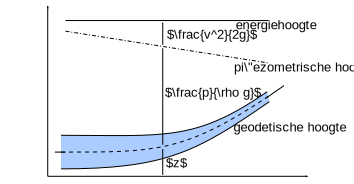
\includegraphics{../fig/deeltjesvergelijkingen/Energiehoogte}
	\end{frame}
%%%%%%%%%%%%%%%%%%%%%%%%%%%%%%%%%%%%%%%%%%%%%%%%%%%%%%%%%%%%%%%%%%%%%%%%%%%
	\begin{frame}
		\frametitle{Toepassing}
		\vspace{1cm}
		\center
		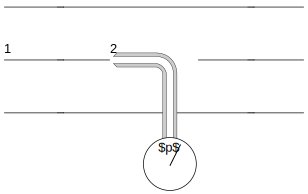
\includegraphics{../fig/deeltjesvergelijkingen/Pitotbuis}
		% met demo
	\end{frame}
%%%%%%%%%%%%%%%%%%%%%%%%%%%%%%%%%%%%%%%%%%%%%%%%%%%%%%%%%%%%%%%%%%%%%%%%%%%
\end{document}			